\subsubsection{Quarto periodo (7/1/2024 - 15/1/2024)}
\subsubsubsection{Planning}
\subsubsubsubsection*{Attività pianificate}
All'inizio del periodo ad ogni membro del gruppo sono stati assegnati ruoli specifici, di seguito riportati:
\begin{table}[H]
\centering
\begin{tabular}{|c|c|c|}
\hline
\textbf{Membro} & \textbf{Ruolo} \\
\hline
Samuele V. & Analista \\
\hline
Michele Z. & Amministratore \\
\hline
Leonardo B. & Responsabile \\
\hline
Riccardo Z. & Programmatore \\
\hline
Filippo T. & Verificatore \\
\hline
Davide B. & Analista \\
\hline
\end{tabular}
\caption{Ruoli assunti per ciascun membro del team all'inizio del periodo}
\end{table}


Gli obiettivi posti per lo $\textit{sprint}_G$ sono stati i seguenti:
\begin{itemize}
    \item Delineare una prima versione del \emph{Piano di Progetto};
    \item Continuare ad aggiornare il documento \emph{Norme di progetto};
    \item Iniziare a sviluppare il \emph{PoC}; 
    \item Continuare la stesura di \emph{Analisi dei Requisiti};
    \item Normare in modo più dettagliato i $\textit{processi organizzativi}_G$;
    \item Richiedere un incontro con il proponente per discutere dei requisiti funzionali trovati mediante i casi d'uso;
    \item Iniziare la stesura del glossario tecnico.
\end{itemize}
\subsubsubsubsection*{Preventivo}
\begin{table}[H]
    \centering
\begin{spreadtab}{{tabular}{|c|c|c|c|c|c|c|c|}}
    \hline
    @\textbf{Membro} & @\textbf{Re} & @\textbf{Amm} & @\textbf{An} & @\textbf{Progr} & @\textbf{Proge} & @\textbf{Ve} & @\textbf{Totale} \\
    \hline
    @ Samuele V.   & 0          & 0          & 4         & 0          & 0     & 0     & sum(b2:g2) \\
    @ Leonardo B.  & 2         & 0          & 0        & 0        & 0     & 2    & sum(b3:g3) \\
    @ Riccardo Z.  & 0          & 0          & 0          & 4          & 0     & 0   & sum(b4:g4) \\
    @ Davide B.    & 0          & 0          & 5       & 0       & 0     & 0     & sum(b5:g5) \\
    @ Michele Z.   & 0          & 4          & 0         & 0          & 0     & 0     & sum(b6:g6) \\
    @ Filippo T.   & 0          & 0          & 0         & 0          & 0     & 3     & sum(b7:g7) \\
    \hline
    @\textbf{Ore totali} & sum(b2:b7) & sum(c2:c7) & sum(d2:d7) & sum(e2:e7) & sum(f2:f7) & sum(g2:g7) &  sum(b8:g8)\\
    \hline
    @\textbf{Costo totale} & 30*b8 & 20*c8 & 25*d8 & 15*e8 & 25*f8 & 15*g8 & sum(b9:g9)\\
    \hline
\end{spreadtab}
    \caption{Preventivo orario ed economico parziale per il quarto periodo, in base al ruolo}
    \label{tab:prev_rtb}
    \vspace{5mm}
    \textbf{Legenda:} \textit{Re} = Responsabile, \textit{Amm} = Amministratore, \textit{An} = Analista, \textit{Progr} = Programmatore, \textit{Proge} = Progettista, \textit{Ve} = Verificatore
\end{table}

\begin{figure}[H]
  \centering
  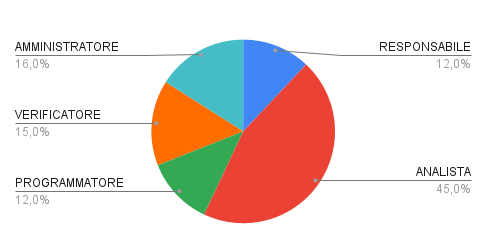
\includegraphics[width=0.6\linewidth]{grafici/4_periodo_torta.png}
  \caption{Ripartizione dei costi per ruolo nel $4^\circ$ periodo}
        \vspace{10mm}
  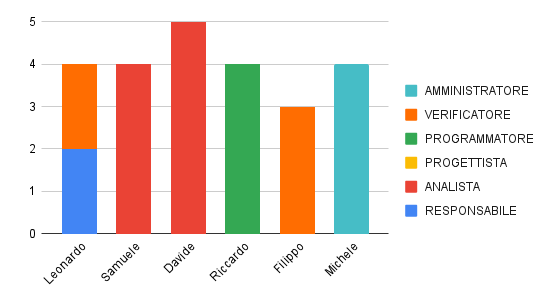
\includegraphics[width=0.7\linewidth]{grafici/4_periodo_istogramma.png}
  \caption{Ore preventivate per ciascuna persona nel $4^\circ$ periodo}
\end{figure}


\subsubsubsection{Review}
\subsubsubsubsection*{Attività svolte}
Periodo di assestamento causa sessione di esami.
Sono state prese le seguenti decisioni:
\begin{itemize}
    \item Utilizzo del $\textit{software}_G$ \emph{Jira} per assegnare le issues e tenere conto del tracciamento temporale di ognuna di esse;
    \item Utilizzo del modello di sviluppo \emph{Scrum};
    \item Utilizzo di linee guida per il documento di \emph{Analisi dei Requisiti} in merito allo stile da adottare nell'uso dei diagrammi e nella specifica testuale dei casi d'uso.
\end{itemize}
\subsubsubsubsection*{Consuntivo}
\begin{table}[H]
    \centering
\begin{spreadtab}{{tabular}{|c|c|c|c|c|c|c|c|}}
    \hline
    @\textbf{Membro} & @\textbf{Re} & @\textbf{Amm} & @\textbf{An} & @\textbf{Progr} & @\textbf{Proge} & @\textbf{Ve} & @\textbf{Totale} \\
    \hline
    @ Samuele V.   & 0          & 0          & 3         & 0          & 0     & 0     & sum(b2:g2) \\
    @ Leonardo B.  & 1.25         & 0          & 1.5        & 0        & 0     & 2    & sum(b3:g3) \\
    @ Riccardo Z.  & 0          & 0          & 0          & 3.5          & 0     & 0   & sum(b4:g4) \\
    @ Davide B.    & 0          & 0          & 3.5       & 0       & 0     & 0     & sum(b5:g5) \\
    @ Michele Z.   & 0          & 3        & 0         & 0          & 0     & 0     & sum(b6:g6) \\
    @ Filippo T.   & 0          & 0          & 0         & 0          & 0     & 3     & sum(b7:g7) \\
    \hline
    @\textbf{Ore totali} & sum(b2:b7) & sum(c2:c7) & sum(d2:d7) & sum(e2:e7) & sum(f2:f7) & sum(g2:g7) &  sum(b8:g8)\\
    \hline
    @\textbf{Costo totale} & 30*b8 & 20*c8 & 25*d8 & 15*e8 & 25*f8 & 15*g8 & sum(b9:g9)\\
    \hline
    %@\textbf{Diff. preventivo} & 0 & -1 & -7 & 0 & 0 & 0 & sum(b10:g10)\\
    %\hline
\end{spreadtab}
    \caption{Preventivo orario ed economico parziale per il quarto periodo, in base al ruolo}
    \label{tab:prev_rtb}
    \vspace{5mm}
    \textbf{Legenda:} \textit{Re} = Responsabile, \textit{Amm} = Amministratore, \textit{An} = Analista, \textit{Progr} = Programmatore, \textit{Proge} = Progettista, \textit{Ve} = Verificatore
\end{table}
\subsubsubsection{Retrospective}
\subsubsubsubsection*{Rischi verificati}
I $\textit{rischi}_G$ riscontrati in questa fase sono stati: \nameref{ro:3},\nameref{ro:4}
Ci sono stati rallentamenti nell'avanzamento dei lavori e difficoltà nel coordinamento delle attività causa l'imminente sessione d'esame. Sono stati risolti, almeno parzialmente, i problemi di tracciamento delle ore tramite l'uso dello $\textit{strumento}_G$ \emph{Jira}.